\documentclass[hidelinks,12pt]{article}
\usepackage[left=0.25cm,top=1cm,right=0.25cm,bottom=1cm]{geometry}
%\usepackage[landscape]{geometry}
\textwidth = 20cm
\hoffset = -1cm
\usepackage[utf8]{inputenc}
\usepackage[spanish,es-tabla]{babel}
\usepackage[autostyle,spanish=mexican]{csquotes}
\usepackage[tbtags]{amsmath}
\usepackage{nccmath}
\usepackage{amsthm}
\usepackage{amssymb}
\usepackage{mathrsfs}
\usepackage{graphicx}
\usepackage{subfig}
\usepackage{standalone}
\usepackage[outdir=./Imagenes/]{epstopdf}
\usepackage{siunitx}
\usepackage{physics}
\usepackage{color}
\usepackage{float}
\usepackage{hyperref}
\usepackage{multicol}
%\usepackage{milista}
\usepackage{anyfontsize}
\usepackage{anysize}
%\usepackage{enumerate}
\usepackage[shortlabels]{enumitem}
\usepackage{capt-of}
\usepackage{bm}
\usepackage{relsize}
\usepackage{placeins}
\usepackage{empheq}
\usepackage{cancel}
\usepackage{wrapfig}
\usepackage[flushleft]{threeparttable}
\usepackage{makecell}
\usepackage{fancyhdr}
\usepackage{tikz}
\usepackage{bigints}
\usepackage{scalerel}
\usepackage{pgfplots}
\usepackage{pdflscape}
\pgfplotsset{compat=1.16}
\spanishdecimal{.}
\renewcommand{\baselinestretch}{1.5} 
\renewcommand\labelenumii{\theenumi.{\arabic{enumii}})}
\newcommand{\ptilde}[1]{\ensuremath{{#1}^{\prime}}}
\newcommand{\stilde}[1]{\ensuremath{{#1}^{\prime \prime}}}
\newcommand{\ttilde}[1]{\ensuremath{{#1}^{\prime \prime \prime}}}
\newcommand{\ntilde}[2]{\ensuremath{{#1}^{(#2)}}}

\newtheorem{defi}{{\it Definición}}[section]
\newtheorem{teo}{{\it Teorema}}[section]
\newtheorem{ejemplo}{{\it Ejemplo}}[section]
\newtheorem{propiedad}{{\it Propiedad}}[section]
\newtheorem{lema}{{\it Lema}}[section]
\newtheorem{cor}{Corolario}
\newtheorem{ejer}{Ejercicio}[section]

\newlist{milista}{enumerate}{2}
\setlist[milista,1]{label=\arabic*)}
\setlist[milista,2]{label=\arabic{milistai}.\arabic*)}
\newlength{\depthofsumsign}
\setlength{\depthofsumsign}{\depthof{$\sum$}}
\newcommand{\nsum}[1][1.4]{% only for \displaystyle
    \mathop{%
        \raisebox
            {-#1\depthofsumsign+1\depthofsumsign}
            {\scalebox
                {#1}
                {$\displaystyle\sum$}%
            }
    }
}
\def\scaleint#1{\vcenter{\hbox{\scaleto[3ex]{\displaystyle\int}{#1}}}}
\def\bs{\mkern-12mu}


\title{Oscilaciones en una membrana circular \\ \large {Funciones de Bessel - Funciones especiales} \vspace{-3ex}}
\author{M. en C. Gustavo Contreras Mayén}
\date{ }

\pagestyle{fancy}
\fancyhf{}
\rhead{Curso MAF}
\lhead{\leftmark}
\rfoot{\thepage}
\setlength{\headheight}{16pt}%

\def\changemargin#1#2{\list{}{\rightmargin#2\leftmargin#1}\item[]}
\let\endchangemargin=\endlist 


\begin{document}
\maketitle
\fontsize{14}{14}\selectfont
\tableofcontents
\newpage

\section{Marco teórico.}
\subsection{Introducción.}

Consideramos ondas estacionarias en un sistema bidimensional con simetría circular:  la de una membrana circular delgada y flexible (por ejemplo, un parche circular de tambor idealizado) de radio $R$.
\par
La ecuación de onda en coordenadas cilíndricas en dos dimensiones $(x , y \to r, \varphi)$ para la amplitud del desplazamiento, $\psi (r, \varphi, t)$ viene dada por:
\begin{align*}
\laplacian{\psi} (r, \varphi, t) - \dfrac{1}{v^{2}} \, \pdv[2]{\psi (r, \varphi, t)}{t} = 0
\end{align*}
Donde la velocidad longitudinal de propagación de ondas transversales en una membrana circular bidimensional estirada está (también) dada por:
\begin{align*}
v = \sqrt{\dfrac{T_{\ell}}{\sigma}}
\end{align*}
donde:
\begin{enumerate}[label=\alph*)]
\item $T_{\ell}$ es la tensión superficial de la membrana (en $\si{\newton\per\metre}$).
\item $\sigma \equiv M/A = M / \pi \, R^{2}$ es la densidad de masa superficial de la membrana (en $\si{\kilo\gram\per\square\metre}$).
\end{enumerate}

Con las reglas de transformación del sistema cartesiano al cilíndrico en 2D:
\begin{align*}
x &= r \, \cos \varphi \\[0.5em]
y &= r \, \sin \varphi \\[0.5em]
\dd[2]{r} &= r \, \dd{r} \dd{\varphi}
\end{align*}
El operador Laplaciano, $\laplacian$ en coordenadas cilíndricas en 2D viene dado por:
\begin{align*}
\laplacian = \dfrac{1}{r} \, \pdv{r} \left( r \, \pdv{r} \right) + \dfrac{1}{r^{2}} \, \pdv[2]{\phi}
\end{align*}

Así, la ecuación de onda bidimensional que describe el comportamiento de las ondas en una membrana cilíndrica viene dada por:
\begin{align*}
\pdv[2]{\psi}{r} + \dfrac{1}{r} \pdv{\psi}{r} + \dfrac{1}{r^{2}} \, \pdv[2]{\psi}{\varphi} = \dfrac{1}{v^{2}} \, \pdv[2]{\psi}{t}
\end{align*}

Notemos que el lado izquierdo de la igualdad (lado derecho de la igualdad) contiene solo funciones dependientes del espacio (dependientes del tiempo), respectivamente.

\section{Separación de variables.}
\subsection{Solución propuesta.}

Por lo tanto, podemos usar la técnica de separación de variables, proponiendo una solución a la ecuación, de la forma:
\begin{align*}
\psi (r, \varphi, t) = U(r, \varphi) \, T(t)
\end{align*}
donde $U (r, \varphi)$ contiene solo términos espacialmente dependientes de $r$ y $\varphi$ y $T (t)$ contiene solo el término dependiente del tiempo.

Tenemos la conocida relación entre la velocidad, la frecuencia y longitud de onda:
\begin{align*}
v &= f \lambda = \left( \dfrac{\omega}{2 \, \pi} \right) \left( \dfrac{2 \, \pi}{k} \right) = \dfrac{\omega}{k}
\end{align*}
entonces $v \, k = \omega$.

Obtenemos una constante de separación $-k^{2}$, y después de realizar algunas manipulaciones algebraicas simples, llegamos a las siguientes ED2H:
\begin{align*}
\pdv[2]{\psi}{r} + \dfrac{1}{r} \pdv{\psi}{r} + \dfrac{1}{r^{2}} \, \pdv[2]{\psi}{\varphi} + k^{2} \, U(r, \varphi) &= 0\\[0.5em]
\dv[2]{T(t)}{t} + \omega \, T(t) &= 0
\end{align*}

Podemos usar nuevamente la técnica de separación de variables en la ecuación espacial anterior,  con una solución de producto de la forma:
\begin{align*}
U(r, \varphi) = R(r) \, \Phi (\varphi)
\end{align*}

Incorporando este producto en la ecuación espacial anterior y realizando las diferenciaciones (parciales),  dividiendo por $U(r, \varphi)$ y realizando nuevamente una manipulación algebraica simple,  obtenemos la siguiente ecuación:
\begin{align*}
\dfrac{1}{R} \left( r^{2} \, \dv[2]{R}{r} +  r \, \dv{R}{r} + k^{2} \, r^{2} \, R(r) \right) = - \dfrac{1}{\Phi} \, \dv[2]{\Phi}{\varphi}
\end{align*}
El lado izquierdo de la igualdad (el lado derecho) de esta ecuación depende solo de $r$ (solo de $\varphi$), respectivamente.
\par
Nuevamente, esto solo puede ser cierto para todos los valores posibles de $(r, \varphi)$, si tanto el lado izquierdo de la expresión como el lado derecho, son iguales a una constante (adimensional).


\subsection{Soluciones periódicas.}

Sabemos que las soluciones $\Phi(\varphi)$ deben ser periódicas y univaluadas, es decir:
\begin{align*}
\Phi (\varphi = 0) = \Phi (\varphi = 2 \, \pi)
\end{align*}
De manera general:
\begin{align*}
\Phi (\varphi = \varphi_{0}) &= \Phi (\varphi = \varphi_{0} + 2 \, m \, \pi), \\[0.em]
&m = 0, \pm 1, \pm 2,\pm 3, \ldots
\end{align*}
Por lo tanto, elegiremos esta constante de separación para que sea $m^{2}$.
\par
Las eigenfunciones de $\Phi_{m} (\varphi)$ son (una de) las dos siguientes formas equivalentes:
\begin{align*}
\Phi_{m} (\varphi) &= \alpha_{m} \, \cos m \, \varphi + \beta \, \sin m \, \varphi \\[1em]
&\begin{cases}
-1 \leq \alpha_{m} \leq 1, \\
-1 \leq \beta_{m} \leq 1 \\
\sqrt{\alpha_{m}^{2} + \beta_{m}^{2}} = 1
\end{cases}
\end{align*}

La segunda forma es:
\begin{align*}
\Phi_{m} (\varphi) &= \exp\big[ i (m \, \varphi + \delta_{m}) \big] \hspace{0.6cm} \delta_{m} = \tan^{-1} \left( \dfrac{\beta_{m}}{\alpha_{m}}\right) \\[1em]
&\mbox{con } m = 0, \pm 1, \pm 2, \ldots
\end{align*}

\subsection{Ecuación de Bessel.}

La ecuación radial es la conocida ecuación diferencial de Bessel:
\begin{align*}
\dv[2]{R}{r} + \dfrac{1}{r} \, \dv{R}{r} + \left( k^{2} - \dfrac{m^{2}}{r^{2}} \right) \, R = 0
\end{align*}

La solución más general a la ecuación de Bessel, con $m$ entero (que es el caso que aquí tenemos), es de la forma:
\begin{align*}
R_{m} (r) = A_{m} \, J_{m} (k \, r) + B_{m} \, Y_{m} (k \, r)
\end{align*}
donde $J_{m} (x)$ son las funciones ordinarias de Bessel de orden $m$, y las $Y_{m} (x)$ son las funciones de Bessel de segundo orden.
\par
Las funciones $J_{m} (x)$ son finitas en $x = 0$ y se expresan normalmente en términos de una serie de potencias en $x$:
\begin{align*}
J_{m} (x) = \sum_{r=0}^{\infty} \dfrac{(-1)^{r}}{r! \, \Gamma(m + r + 1)} \, \left( \dfrac{x}{2} \right)^{m+2r}
\end{align*}

Sabemos que para $m$ entero: $J_{-m} (x) = (-1)^{m} \, J_{m} (x)$.
\par
Las funciones $Y_{m} (x)$ se pueden expresar de diversas maneras, entre ellas:
\begin{align*}
Y_{m}(x) = \dfrac{J_{m}(x) \, \cos (m \, \pi) - J_{-m}(x)}{\sin (m \, \pi)}
\end{align*}

Para $m$ entero, también se pueden escribir como:
\begin{align*}
Y_{m}(x) = \dfrac{1}{\pi} \left[ \pdv{J_{m}(x)}{m} - (-1)^{m} \, \pdv{J_{-m}(x)}{m} \right]
\end{align*}

Las funciones $Y_{m} (x)$ son singulares (se vuelven (negativas) infinitas) en $x = 0$. Sin embargo, debido a que usamos coordenadas cilíndricas para nuestra membrana circular, el origen $(r = 0)$ \textbf{se incluye} en este problema.
\par
Físicamente, \textbf{NO} se permiten desplazamientos de amplitud infinitos tal que $R(r) \to \infty$ para cualquier valor de $r$, ya que una suposición inicial implícita eran oscilaciones de \emph{amplitud pequeñas}. 
\par
Por tanto, todos los coeficientes $B_{m}$ para el $Y_{m} (x)$ deben ser $B_{m} = 0$ para soluciones en valores propios físicamente permitidas de la membrana circular bidimensional.
\par
La condición de frontera radial para ondas estacionarias transversales en una membrana circular con borde fijo (es decir, desplazamiento transversal cero) en $r = R$ es $R_{m} (r = R) = 0$,  es decir, $J_{m} (k \, R) = 0$.
\par
Dado que $r = R > 0$, esto significa que buscamos los ceros de $J_{m} (k \, R)$, es decir, $J_{m} (x = k \,R) = 0$. Debido a la complejidad de la forma de $J_{m} (x)$, los ceros de $J_{m} (x)$ (y $Y_{m} (x)$) son de naturaleza no analítica, más bien, están tabulados en muchos libros de matemáticas, o pueden determinarse mediante técnicas numéricas gráficas y/o computacionales.
\par
Presentamos los primeros ceros del $J_{m} (x)$ de orden inferior en la siguiente tabla:
\begin{table}[H]
\centering
\begin{tabular}{c c c c c c}
    & & & $n=1$ & $n=2$ & $n=3$ \\
$m=0:$ & $J_{0}(x)=0:$ & $x \approx$ & $2.40$ & $5.52$ & $8.65  \ldots$ \\
$m=1:$ & $J_{1}(x)=0:$ & $x \approx$ & $3.83$ & $7.02$ & $10.17 \ldots$ \\
$m=2:$ & $J_{2}(x)=0:$ & $x \approx$ & $5.14$ & $8.42$ & $11.62 \ldots$ \\
\vdots
\end{tabular}
\end{table}

Dado que $x = k \, R$, entonces $k = x / R$ y observando nuevamente, para este problema de eigenvalores de onda estacionaria bidimensional, \textbf{tenemos dos índices}: $m$ y $n$ para denotar:
\begin{enumerate}[label=\alph*)]
\item Los eigenvalores de onda $k_{m, n}= x_{m, n} / R$,
\item Las eigenfrecuencias $\omega_{m, n}  = v \, k_{m, n}$  $f_{m, n} = v / \lambda_{m, n}$ con $v = \sqrt{T_{\ell} / \sigma}$,
\item Las eigenenergías, $E_{m, n} = \dfrac{1}{4} M \, \omega_{m, n}^{2} \, A_{m, n}^{2}$
\item Las eigenfunciones $\psi_{m, n} (r, \varphi, t) = R_{m,n} (r) \, \Phi_{m} (\varphi) \, T_{m, n} (t)$
\end{enumerate}

Las soluciones en eigenmodos de la ecuación de onda temporal asociada para ondas estacionarias bidimensionales en una membrana circular son de la siguiente(s) forma(s) equivalente(s):
\begin{align*}
\mathbf{i)} \hspace{0.15cm} T_{m,n} (t) &= b_{m,n} \, \sin (\omega_{m,n} \, t) {+} c_{m,n} \, \cos (\omega_{m,n} \, t) \\[0.5em]
-1 &\leq b_{m,n} \leq 1 \hspace{1cm} -1 \leq c_{m,n} \leq 1 \\[0.5em]
&\sqrt{b_{m,n}^{2} + c_{m,n}^{2}} = 1 \\[0.5em]
\mathbf{ii)} \hspace{0.2cm} T_{m,n} (t) &= \sin (\omega_{m,n} \, t + \delta_{m,n}) = \\[0.5em] 
&= \cos(\omega_{m,n} \, t + \varphi_{m,n}) \\[0.5em] 
\delta_{m,n} = \varphi_{m,n} &+ \dfrac{\pi}{2} \\[0.5em] 
\mathbf{iii)} \hspace{0.2cm} T_{m,n} (t) &= \exp\big[ i(\omega_{m,m} \, t + \varphi_{m,n}) \big]
\end{align*}

\section{Solución completa.}
\subsection{Eigenmodos de vibración.}

Las soluciones completas en eigenmodos para ondas estacionarias bidimensionales en una membrana circular de radio, $R$ con bordes fijos están dadas por alguna de las siguientes expresiones que son equivalentes:
\begin{align*}
\psi_{m,n} (r ,\varphi, t) &= R_{m,n} (r) \, \Phi_{m} (\varphi) \, T_{m,n} (t) \\[0.5em] 
\psi_{m,n} (r ,\varphi, t) &= A_{m,n} \, J_{m,n} (k_{m,n} \, R) \times \\[0.5em]
&\times \exp\big[ i(m \, \varphi + \delta_{m,n}) \big] \, \exp\big[ i(\omega_{m,n} \, t + \varphi_{m,n}) \big] \\[0.5em]
\psi_{m,n} (r ,\varphi, t) &= A_{m,n} \, J_{m,n} (k_{m,n} \, R) \times \\[0.5em]
&\times \big[ \alpha_{m,n} \,  \cos (m \, \varphi) + \beta_{m} \, \sin (m \, \varphi) \big] \times \\[0.5em]
&\times \big[ b_{m,n} \,  \cos (\omega_{m,n} \, t) + c_{m,n} \, \sin (\omega_{m,n} \, t) \big]
\end{align*}   
Con:
\begin{enumerate}[label=\roman*)]
\item Eigenfrecuencias:
\begin{eqnarray*}
f_{m,n} = \dfrac{\omega_{m,n}}{2 \, \pi} =  \dfrac{v \, k_{m,n}}{2 \, \pi} =  \dfrac{v}{\lambda_{m,n}}
\end{eqnarray*}
\item Longitudes de onda propias:
\begin{eqnarray*}
\lambda_{m,n} = \dfrac{2 \, \pi}{k_{m,n}} =  \dfrac{2 \, \pi \, R}{x_{m,n}}
\end{eqnarray*}
\item Eigenenergías:
\begin{align*}
E_{m,n} = \dfrac{1}{4} \, M \, \omega_{m,n}^{2} \, A_{m,n}^{2}
\end{align*}
\begin{align*}
m = 0, 1, 2, 3, \ldots \hspace{1cm} n = 1, 2, 3, \ldots
\end{align*}
\end{enumerate}

\subsection{Modos bajos de vibración.}

Los modos más bajos de ondas estacionarias transversales en una membrana circular se enumeran a continuación:
\begin{table}[H]
\centering
\large
\begin{tabular}{c c c c l}
$m {=} 0$ & $n {=} 1$ & $k_{0,1} {\approx} 2.40/R$ & $\omega_{0,1} {\approx} 2.40 \, v/R$ & \\[0.5em] 
\multicolumn{5}{l}{$\psi_{0,1}(r, \varphi, t) {=} A_{0,1} \, J_{0}(k_{0,1} \, R) \, T_{0,1}(t)$} \\[0.5em] \hline 
$m {=} 1$ & $n {=} 1$ & $k_{1,1} {\approx} 3.83/R$ & $\omega_{1,1} {\approx} 3.83 v/R$ & \\[0.5em]
\multicolumn{5}{l}{$\psi_{1,1}(r, \varphi, t) {=} A_{1,1} J_{1}(k_{1,1} R) \big[ \alpha_{1} \cos \varphi {+} \beta_{1} \sin \varphi \big] T_{0,1}(t)$} \\[0.5em] \hline 
$m {=} 2$ & $n {=} 1$ & $k_{2,1} {\approx} 5.14/R$ & $\omega_{2,1} {\approx} 5.14 v/R$ & \\[0.5em]
\multicolumn{5}{l}{$\psi_{2,1}(r, \varphi, t) {=} A_{2,1} J_{2}(k_{2,1} R) \big[ \alpha_{2} \cos 2 \varphi {+} \beta_{2} \sin 2 \varphi \big] T_{2,1}(t)$} \\[0.5em] \hline
$m {=} 0$ & $n {=} 2$ & $k_{0,2} {\approx} 5.52/R$ & $\omega_{0,1} {\approx} 5.52 \, v/R$ & \\[0.5em]
\multicolumn{5}{l}{$\psi_{0,2}(r, \varphi, t) {=} A_{0,2} \, J_{0}(k_{0,2} \, R) \, T_{0,2}(t)$}
\end{tabular}
\end{table}

\subsection{Visualización.}

Algunos de los modos de vibración propios de orden inferior para ondas estacionarias transversales en una membrana circular (con líneas nodales discontinuas) se muestran a continuación:

\begin{minipage}{0.3\textwidth}
\begin{figure}[H]
    \centering
    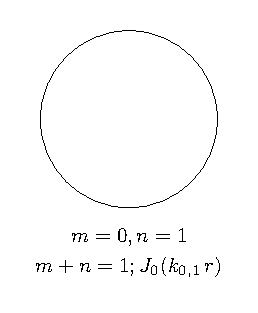
\includegraphics[scale=1]{Imagenes/Modos_Vibracion_Membrana_0_1.eps}
\end{figure}
\end{minipage}
\begin{minipage}{0.3\textwidth}
\begin{figure}[H]
    \centering
    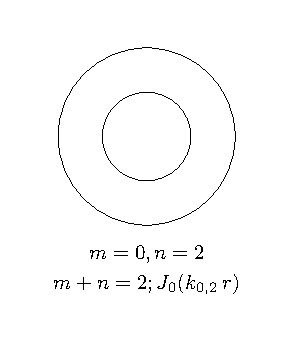
\includegraphics[scale=1]{Imagenes/Modos_Vibracion_Membrana_0_2.eps}
\end{figure}
\end{minipage}
\begin{minipage}{0.3\textwidth}
\begin{figure}[H]
    \centering
    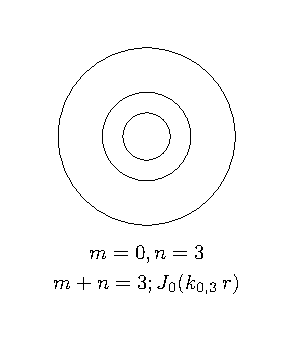
\includegraphics[scale=1]{Imagenes/Modos_Vibracion_Membrana_0_3.eps}
\end{figure}
\end{minipage}

La línea continua indica la región en donde no hay desplazamiento de la membrana, en el caso $m = 0$, $n = 1$, la circunferencia de la misma permanece fija, y el desplazamiento es sobre toda la membrana, en el caso $m = 0$, $n = 2$ se genera una nueva circunferencia y es la que permanece fija, esto implica que la región dentro de ésta, oscila de manera contraria a la región que está por fuera de la circunferencia, de la misma manera ocurre en el caso $m = 0$, $n = 3$, que ahora tiene tres regiones distintas.
\par
Las degeneraciones de orden 2 para $m > 0$ surgen de nuevo debido a los 2 grados espaciales de libertad ($x$ e $y$, $r$ y $\varphi$). La simetría rotacional de la membrana circular: es invariante en rotaciones arbitrarias. A continuación se muestran los modos de vibración para funciones degeneradas:
\begin{minipage}{0.3\linewidth}
\begin{figure}[H]
    \centering
    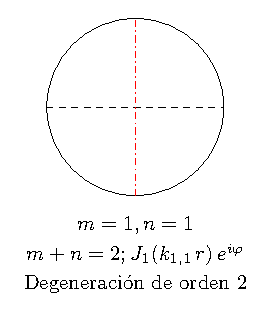
\includegraphics[scale=1]{Imagenes/Modos_Vibracion_Membrana_1_1.eps}
\end{figure}
\end{minipage}
\begin{minipage}{0.3\linewidth}
\begin{figure}[H]
    \centering
    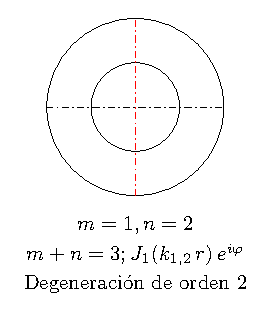
\includegraphics[scale=1]{Imagenes/Modos_Vibracion_Membrana_1_2.eps}
\end{figure}
\end{minipage}
\begin{minipage}{0.3\linewidth}
\begin{figure}[H]
    \centering
    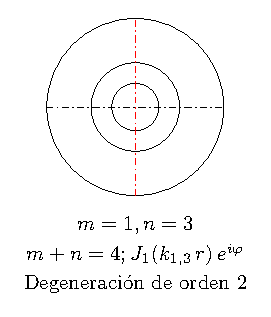
\includegraphics[scale=1]{Imagenes/Modos_Vibracion_Membrana_1_3.eps}
\end{figure}
\end{minipage}

\begin{minipage}{0.3\linewidth}
\begin{figure}[H]
    \centering
    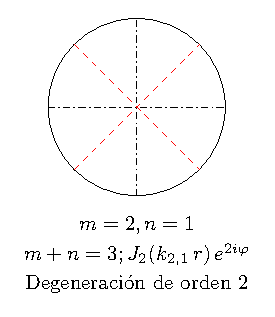
\includegraphics[scale=1]{Imagenes/Modos_Vibracion_Membrana_2_1.eps}
\end{figure}
\end{minipage}
\begin{minipage}{0.3\linewidth}
\begin{figure}[H]
    \centering
    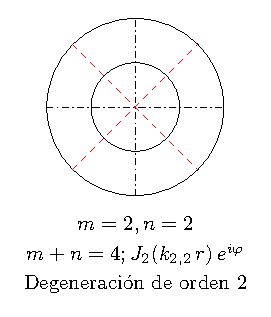
\includegraphics[scale=1]{Imagenes/Modos_Vibracion_Membrana_2_2.eps}
\end{figure}
\end{minipage}
\begin{minipage}{0.3\linewidth}
\begin{figure}[H]
    \centering
    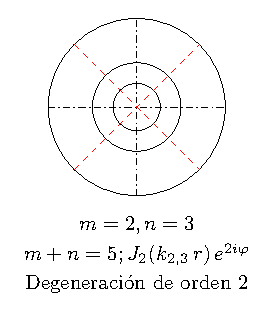
\includegraphics[scale=1]{Imagenes/Modos_Vibracion_Membrana_2_3.eps}
\end{figure}
\end{minipage}

 Una siguiente parte de estudio sobre los modos de vibración de una membrana circular, es sobre la manera de visualizar las oscilaciones. En las figura anteriores, se nota la descripción por zonas en la membrana, para extender el estudio, es ahora necesario el apoyo de herramientas ya sea de programación o de software matemático.
\par
En la siguiente figura se presenta el mismo arreglo descriptivo, pero ahora con más información, se utilizó el software \texttt{Mathematica}, para resolver la ecuación diferencial, obtener los ceros de las funciones de Bessel y finalmente, ocupar una rutina de graficación para visualizar de otra manera el mismo resultado:

\begin{minipage}{0.3\linewidth}
\begin{figure}[H]
    \centering
    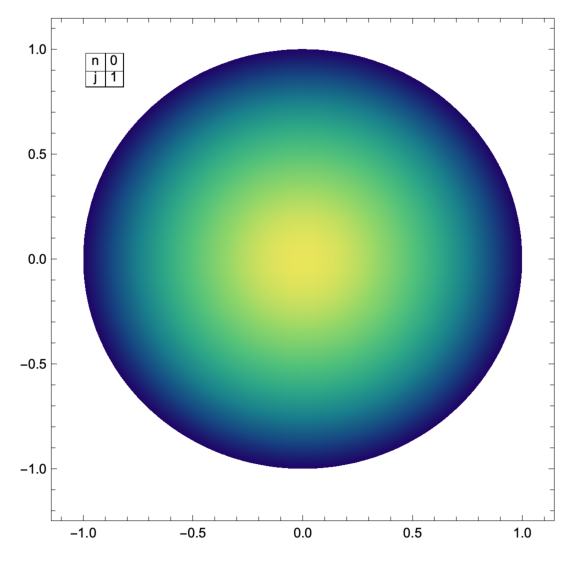
\includegraphics[scale=0.5]{Imagenes/Vibracion_Membrana_01.eps}
\end{figure}
\end{minipage}
\begin{minipage}{0.3\linewidth}
\begin{figure}[H]
    \centering
    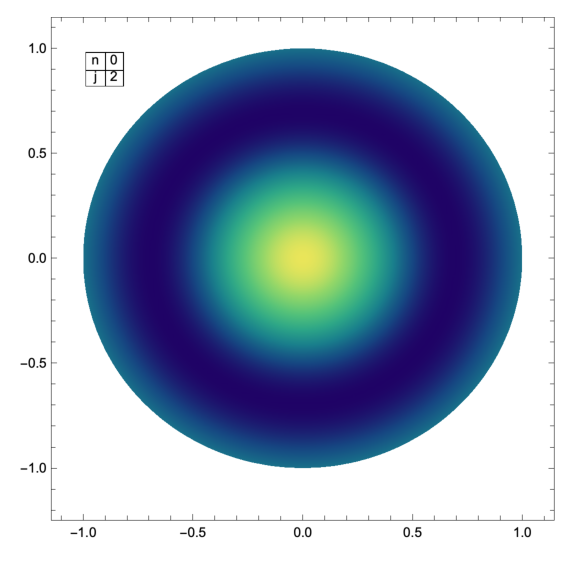
\includegraphics[scale=0.5]{Imagenes/Vibracion_Membrana_02.eps}
\end{figure}
\end{minipage}
\begin{minipage}{0.3\linewidth}
\begin{figure}[H]
    \centering
    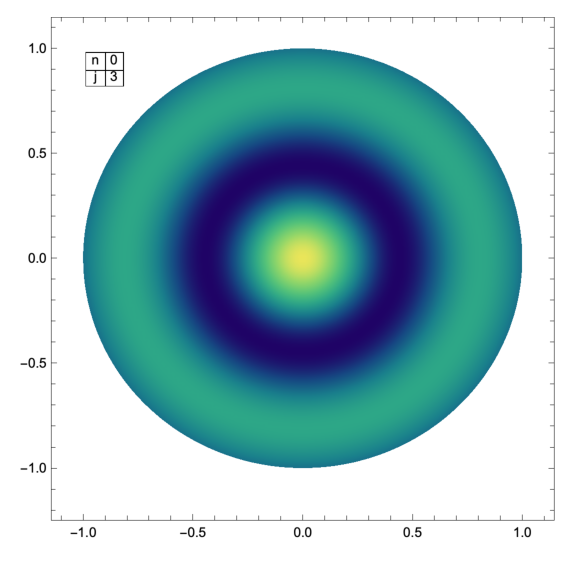
\includegraphics[scale=0.5]{Imagenes/Vibracion_Membrana_03.eps}
\end{figure}
\end{minipage}
\\[0.5em]
Con esta visualización se interpreta que la zona oscura (de color azul) permanece fija, mientras que la zona verde es la que oscila, en el primer recuadro $m = 0$, $n = 1$, sabemos que la circunferencia de la membrana permanece fija, por ello tiene el color azul, mientras que la membrana oscila (color verde), para el caso $m = 0$, $n = 2$, se identifica la nueva circunferencia y se tienen dos regiones distintas, que oscilan en direcciones contrarias.
\end{document}